\section{Telemetry}
\begin{figure}[htb]
	\centering
	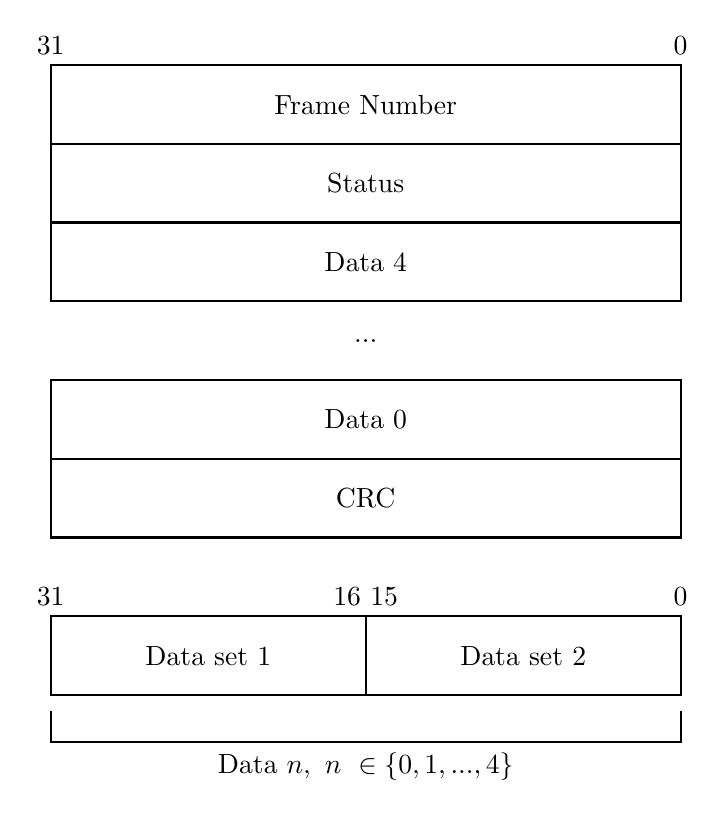
\begin{tikzpicture}
	%\draw [step=1.0,lightgray, very thin] (0.0,0.0) grid (10,10);
	% May move it 
	\draw[thick, black]  (1,10) -- (1,10) node[pos=.5,above] {31};
	\draw[thick, black]  (9,10) -- (9,10) node[pos=.5,above] {0};
	\draw[thick, black] (1, 9) rectangle (9,10) node[pos=.5] {Frame Number};
	\draw[thick, black] (1, 8) rectangle (9,9) node[pos=.5] {Status};
	\draw[thick, white] (1, 6) rectangle (9,7) node[pos=.5, black] {...};
	\draw[thick, black] (1, 7) rectangle (9,8) node[pos=.5] {Data 4};
	\draw[thick, black] (1, 5) rectangle (9,6) node[pos=.5] {Data 0};
	\draw[thick, black] (1, 4) rectangle (9,5) node[pos=.5] {CRC};
	
	\draw[thick, black]  (1,3) -- (1,3) node[pos=.5,above] {31};
	\draw[thick, black]  (5,3) -- (5,3) node[pos=.5,above] {16 15};
	\draw[thick, black]  (9,3) -- (9,3) node[pos=.5,above] {0};
	
	\draw[thick, black] (1, 2) rectangle (5,3) node[pos=.5] {Data set 1};
	\draw[thick, black] (5, 2) rectangle (9,3) node[pos=.5] {Data set 2};
	\draw[thick, black] (1, 1.8) -- (1, 1.4) -- (9, 1.4) node[pos=.5,below]{Data $n, ~n~\in \{0,1,...,4\}$} -- (9, 1.8);
	\end{tikzpicture}
	\caption{Data Frame for telemetry} \label{fig:sp-experimentOverview}
\end{figure}

\noindent There are 18 16-bit-analog-digital-converters (ADC) on both signal processing units. Each ADC is working with up to 2kSPS which leads to a conversion time of $5 \cdot 10^{-4}s$. As we have 2000 samples per second, the data rate of one ADC is 16 times the sample rate, which is 32kbit/s per ADC. Therefore, the total data rate is 576 kbit/s only for the measurement data. The RS-422 connected telemetry system is constrained to handle a data stream with up 30kbit/s for our experiment. So we are not able to send every measured value, uncompressed and in the highest resulotion. To solve this problem, we will select the data to be sent.\\\\
%
The data frame contains a frame number, this one will be generated by the SPU software. The 32 status bit will be used to determine the current health of the system. The bits [17:0(LSB)] are for the adc status bits. 0 ADC ok, 1 adc not ok. The intervall [19:18] will contain two status bits from the MCU. All other bits are reserved.\\\\
%
To handle the data with 32 bit integer values, it is necessary to transmit two values in one 32 bit value. The lower part of \ref{fig:sp-experimentOverview} shows the aligment, when two 16 bit values are being transmitted.\\\\
%
The first three data fields (Data 5 - 3) will be used to transmit the values of all 6 strain gauge rosettes (= 3 STAMPs) connected to the master SPU. Data 2 - 0 contains the temperature for the three connected temperature sensors. The final 16-bit data set 2 of Data 0 will be used for a checksum. The order of the measurement values in the data frame is determined by the STAMP number in ascending order, whereas both rosettes of each rosette is transmitted in two consecutive data frames, beginning with the upper straing gauge rosette.\\\\
%
The header offset is 8 bytes and each full package has 18 bytes of data and 4 byte \texttt{crc}, so one frame is 30 bytes long.\\\\
%
To gather the necessary data we have determine how many packages we are able to send at 30kbit/s. 
$$ N = \frac{30 \frac{kbit}{s}}{240 bit} = 125$$ 
N is the number of frames we are able to send every second. To archive this goal and reach the maximum safe data rating, we need to gather every 16th sample from each ADC. 
$$P = \frac{2000 SPS}{N} = \frac{2000 SPS}{125} = 16 $$
